%TEX root = ../dissertation.tex

\chapter{Architecture}
\label{chapter:architecture}
\section{OpenFlow SDN controller cluster}
\label{section:SDN-controller-cluster}
As previously mentioned, the OpenFlow specification provides mechanisms for resilience and load balancing across multiple \gls{SDN} controller instances.
OpenFlow allows for an OpenFlow switch to be connected to several \gls{SDN} controllers simultaneously, however, the latter are expected to have some sort of coordination between them in order to achieve load balancing, which is achieved by exposing eastbound/westbound \glspl{API} to be consumed by neighboring controllers within the same management domain.
This approach also requires that every OpenFlow switch within the management domain be reconfigure every time an instance is added or removed from the \gls{SDN} controller cluster.\\
%
Having the instances coordinated with each other and keep consistent states in a distributed environment requires therefore a controller cluster and configures an architecture such that of figure \ref{fig:sdn_simple_clustering}.\\
%
\begin{figure}
	\centering
	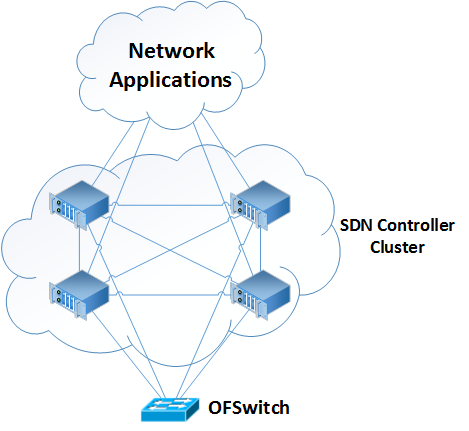
\includegraphics[scale=0.65]{sdn_simple_clustering}
	\caption{OpenFlow SDN controller clustering}
	\label{fig:sdn_simple_clustering}
\end{figure}
%
The resulting cluster should support key aspects of the \gls{SDN} controller component, such as keep a global view and management scope.
Because the goal is to perform load balancing between all instances, each instance will be actively managing any given number of OpenFlow switches in the same management domain, and therefore the network state is distributed in nature.
In order to maintain the aforementioned key aspect of \gls{SDN} controllers, active instances must propagate their \gls{MIB} on to their cluster peers and be prepared to update their own \gls{MIB} with updates issued by their peers.
The propagation of these updates must be triggered at least when network events are detected and when new adjacencies between OpenFlow switches controlled by different instances are detected.
When a instance propagates updates to other peer instances, it must guarantee causal consistency.\\
%
